\documentclass[12pt,a4paper]{article}

\title{LABWORK 4 REPORT}
\author{Ta Hoang Hai Nam - USTHBI6110 \\ Trinh Hoang Hai - USTHBI6047 \\ Le Sinh Quy - USTHBI4127 \\ Kieu Quoc Viet - USTHBI6153 }
\usepackage{listings}
\usepackage{color}
\usepackage{graphicx}
\usepackage[section]{placeins}
\usepackage{float}
\usepackage{amsmath}

\begin{document}
\maketitle
\newpage 
\section{Why Hadoop MapReduce?}
- We choose Hadoop MapReduce because it is the go-to framework for MapReduce.It is very easy to use and it is available for Java.
\section{How?}
\begin{figure}[!h]
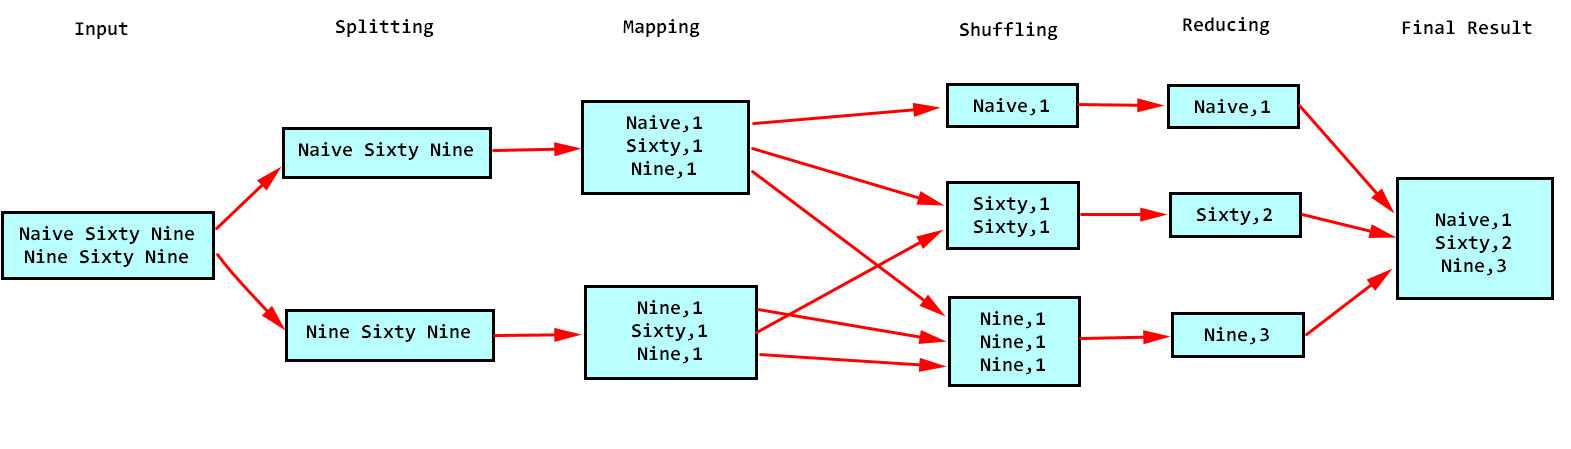
\includegraphics[width=\linewidth]{Mapper_Reducer.jpg}
\caption{How Mapper and Reducer work.}
\end{figure}
Words input to a MapReduce  are broken down and divided into different sentences. 
Then in Mapping step data in each split is gathered to count number of occurrences of each word from input splits and present results in the form of (word, frequency). 
\\ After that,  it will be shuffled into different groups with each group contains the same word. Finally, in the Reducing phase,  the number of output words from Shuffling step and returns the Final result - a single output value. 
\section{Who did what?}
- Code: Ta Hoang Hai Nam \\
- Report: Ta Hoang Hai Nam, Trinh Hoang Hai.
\end{document}